\documentclass[10pt,twocolumn,letterpaper]{article}

\usepackage{cvpr}
\usepackage{times}
\usepackage{epsfig}
\usepackage{graphicx}
\usepackage{amsmath}
\usepackage{amssymb}
% Include other packages here, before hyperref.
% \usepackage[outdir=./]{epstopdf}

% If you comment hyperref and then uncomment it, you should delete
% egpaper.aux before re-running latex.  (Or just hit 'q' on the first latex
% run, let it finish, and you should be clear).
\usepackage[breaklinks=true,bookmarks=false]{hyperref}

% \cvprfinalcopy % *** Uncomment this line for the final submission

\def\cvprPaperID{3510} % *** Enter the CVPR Paper ID here
\def\httilde{\mbox{\tt\raisebox{-.5ex}{\symbol{126}}}}

%% Custom control sequences
\let\oldPr\Pr
\newcommand{\bR}{\mathbb{R}}
\renewcommand*{\Pr}[1]{\mathbb{P}\left( #1 \right)}
\newcommand{\mat}[1]{\mathbf{#1}}
\DeclareMathOperator*{\argmax}{arg\,max}
\DeclareMathOperator*{\argmin}{arg\,min}
\newcommand{\tr}{\mathbf{tr}}
\newcommand{\cross}[1]{[#1]_{\times}}


% Pages are numbered in submission mode, and unnumbered in camera-ready
%\ifcvprfinal\pagestyle{empty}\fi
\setcounter{page}{9}
\begin{document}

%%%%%%%%% TITLE
% \title{All Graphs Lead to Rome: \\
% Cycle Consistent Multi-View Representations Using Graph CNNs}
\title{All Graphs Lead to Rome: Learning Geometric and Cycle-Consistent Representations with Graph Convolutional Networks \\
Supplemental Material}

\author{Stephen Phillips, Kostas Daniilidis \\
GRASP Laboratory, University of Pennsylvania\\
{\tt\small \{stephi, kostas\}@seas.upenn.edu}
% For a paper whose authors are all at the same institution,
% omit the following lines up until the closing ``}''.
% Additional authors and addresses can be added with ``\and'',
% just like the second author.
% To save space, use either the email address or home page, not both
% \and
% Second Author\\
% Institution2\\
% First line of institution2 address\\
% {\tt\small secondauthor@i2.org}
}

% When placing figures in \LaTeX, it's almost always best to use
% \verb+\includegraphics+, and to specify the  figure width as a multiple of
% the line width as in the example below
% {\small\begin{verbatim}
%    \usepackage[dvips]{graphicx} ...
%    \includegraphics[width=0.8\linewidth]
%                    {myfile.eps}
% \end{verbatim}
% }


\maketitle
%\thispagestyle{empty}

% Papers, excluding the references section,
% must be no longer than eight pages in length. The references section
%%%%%%%%% BODY TEXT
\section*{A. Relative Efficiency Against Optimization Based Methods}

In figure \ref{fig:iterplot} we show a more fine grained comparison of our algorithm to optimization based methods at different numbers of iterations.
We show the mean and standard devation of the errors of all methods, testing the optimization based methods at different iterations.


%------------------------------------------------------------------------
\begin{figure*}[ht]
\begin{center}
  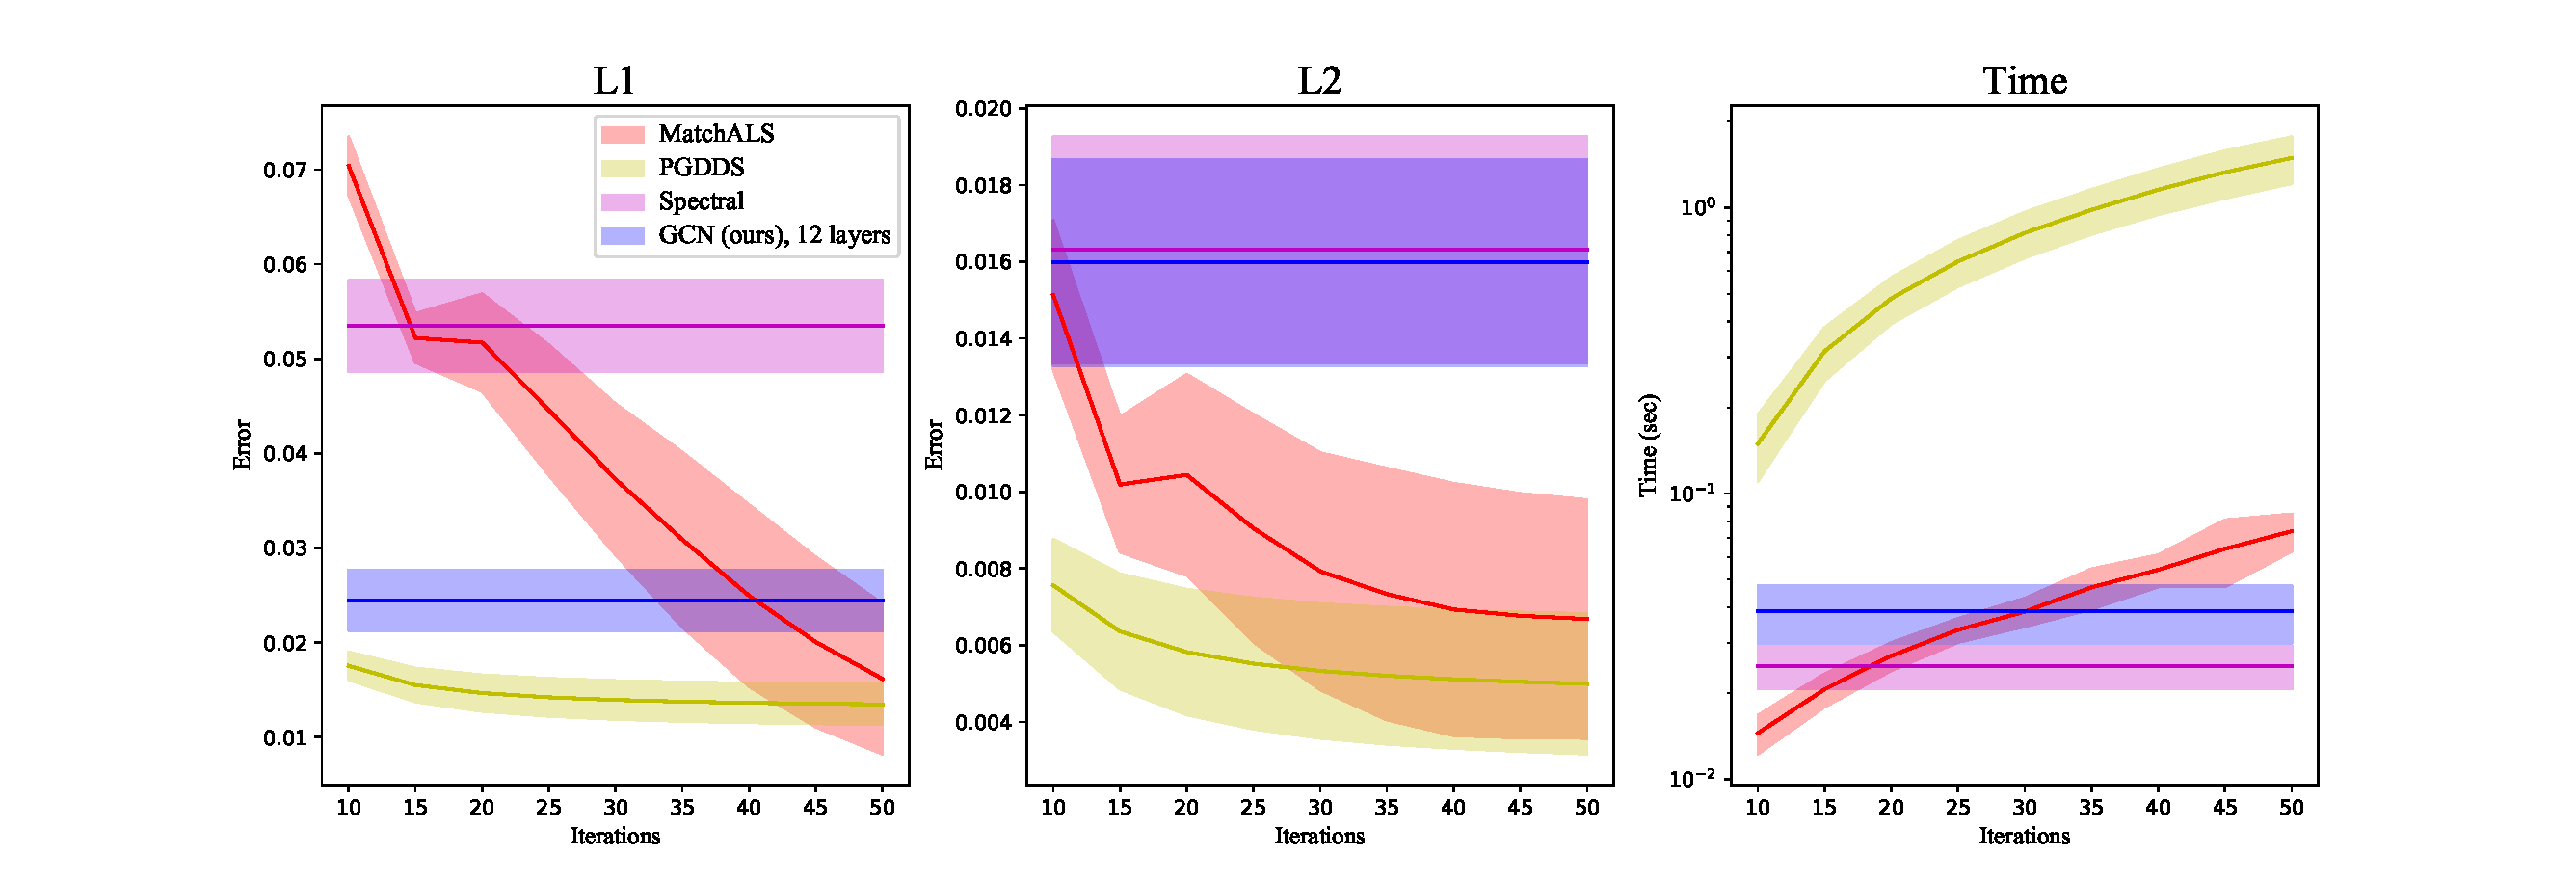
\includegraphics[width=0.9\linewidth]{figures/IterationsPlot.pdf}
\end{center}
  \caption{
    This figure plots the average accuracy of the optimization methods by iteration compared to 12 iterations of our GCN based method.
    The bold center line shows the mean, the colored in region shows 1 standard devation of the errors.
    As we optimize for $L_1$ error, our method's $L_1$ loss is substantially better than its $L_2$ losses.
    The right most plot shows time, plotted on a log scale for clarity.
  }
\label{fig:iterplot}
\label{fig:onecol}
\end{figure*}

\section*{B. Effect of Group Normalization}
We observe that training with group normalization helps with training and generalization error, as shown in figure \ref{fig:groupnorm}.
As the Group Normalization operation is not easily parallelized across nodes in the graph, the use of Group Normalization is the main barrier to parallelization.
Thus we will need to find alternative more parallelizable methods to improve generalization error for future work.

%------------------------------------------------------------------------
\begin{figure*}[ht]
\begin{center}
  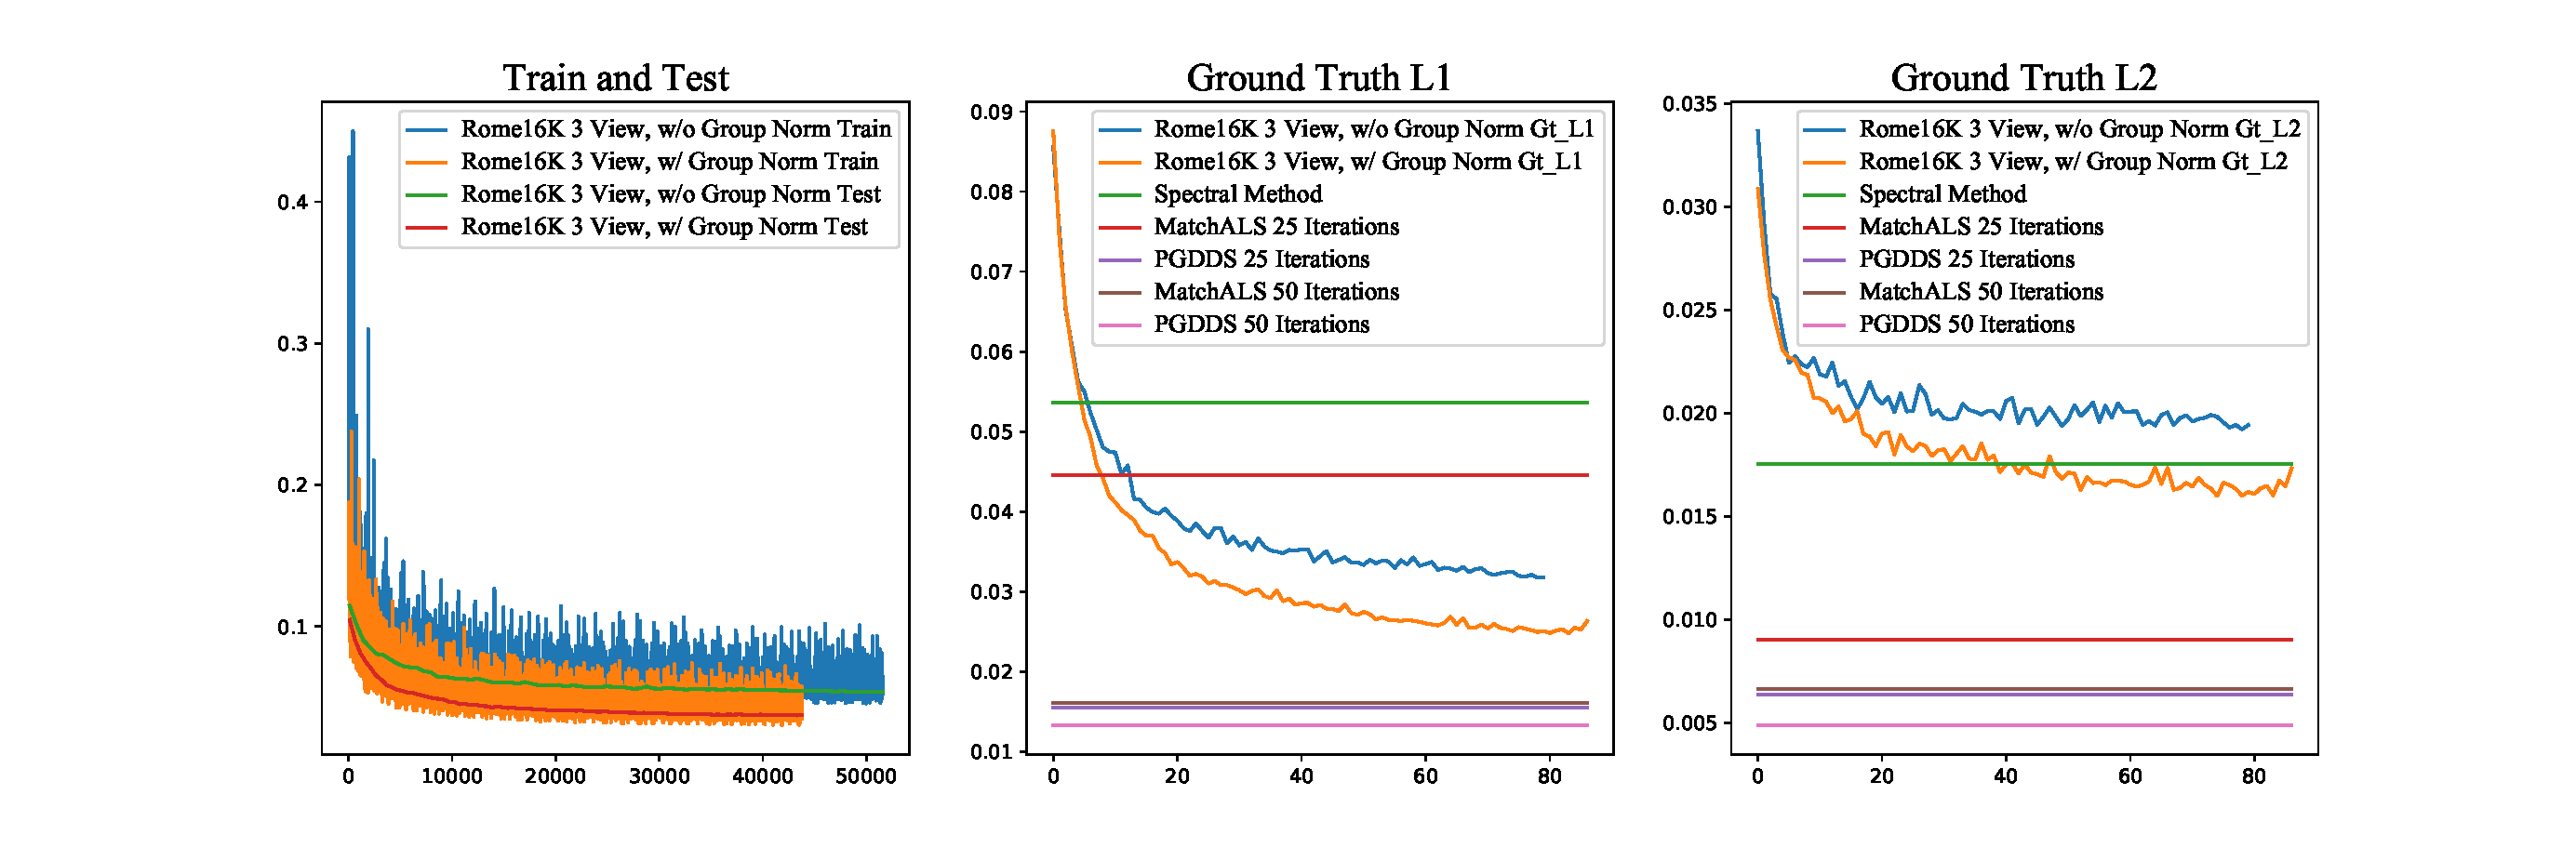
\includegraphics[width=0.9\linewidth]{figures/GroupNormTest.pdf}
\end{center}
  \caption{
    This figure plots the training curves of the network with and without Group Normalization.
    Note that while the train/test curves are fairly similar with or without Group Normalization, distance to the ground truth is improved greatly with Group Normalization.
  }
\label{fig:groupnorm}
\label{fig:onecol}
\end{figure*}


\end{document}
